\begin{frame}
  \frametitle{Installation alternatives}

  % FEniCS uses standard setup.py and cmake tools
  % but dependencies are tricky to configure.

  \begin{tabular}{cp{10cm}}
    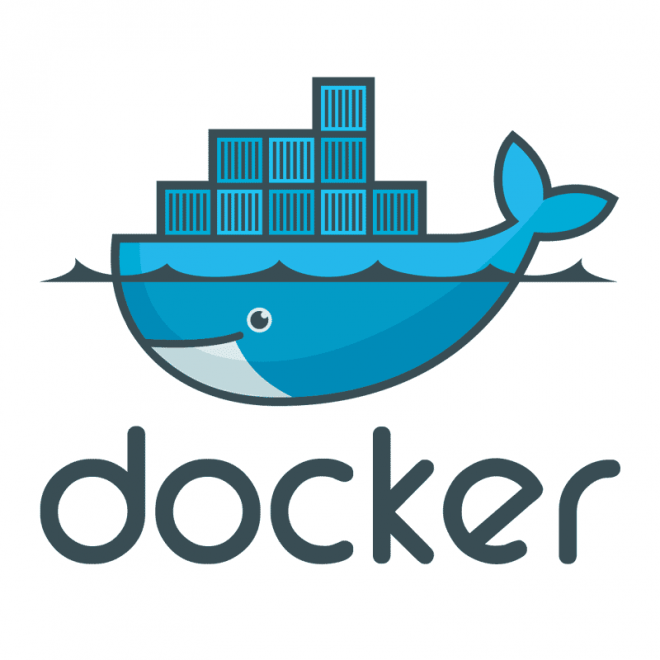
\includegraphics[height=1cm]{png/docker_logo.png} &
    \begin{minipage}{10cm}
      \ding{43} Docker images on Linux, Mac, Windows
      \vspace{0.6cm}
    \end{minipage}
    \\
    
\includegraphics[height=1cm]{png/source.png} &
    \begin{minipage}{10cm}
      \ding{43} Build from source with Hashdist (fenics-install.sh)
      \vspace{0.8cm}
    \end{minipage}
    \\
    
\includegraphics[height=1cm]{png/ubuntu_logo.png} &
    \begin{minipage}{10cm}
      \ding{43} PPA with apt packages for Debian and Ubuntu
      \vspace{0.6cm}
    \end{minipage}
    \\
    
\includegraphics[height=1cm]{png/mac_osx_logo.png} &
    \begin{minipage}{10cm}
      \ding{43} Drag and drop installation on Mac OS X
      \vspace{0.8cm}
    \end{minipage}
  \end{tabular}

  \begin{center}
    \colemph{\url{http://fenicsproject.org/download/}}
  \end{center}

\end{frame}
